\chapter{Veröffentlichung im Play Store\label{chap5:Fuenftes-Kapitel}}

Ziel war neben der Implementierung der mobilen Anwendung \glqq Geogram\grqq{} auch die Veröffentlichung der gleichen App im Google Play Store. Um rechtliche Problematiken bezüglich der Ähnlichkeit zu der App \glqq Instagram\grqq{} vorzubeugen, wurden an der App \glqq Geogram\grqq{} Änderungen vorgenommen.

Eine Änderung bezieht sich auf das verwendete Logo der App \glqq Geogram\grqq{}. In \autoref{fig:oldlogovsnewlogo} ist oben links das alte App-Logo zu erkennen. Verglichen mit dem Instagram-Logo (rechte Seite) ist eine Ähnlichkeit deutlich zu erkennen. Als Gruppe hat man sich deshalb dafür entschlossen ein neues Logo für die App \glqq Geogram\grqq{} zu entwerfen. Das neue Logo der App \glqq Geogram\grqq{} ist in \autoref{fig:oldlogovsnewlogo} unten links abgebildet. Es gibt nun keine Verwechslungsgefahr mehr mit dem Logo der App \glqq Instagram\grqq{}.

\begin{figure}[H]
    \centering
    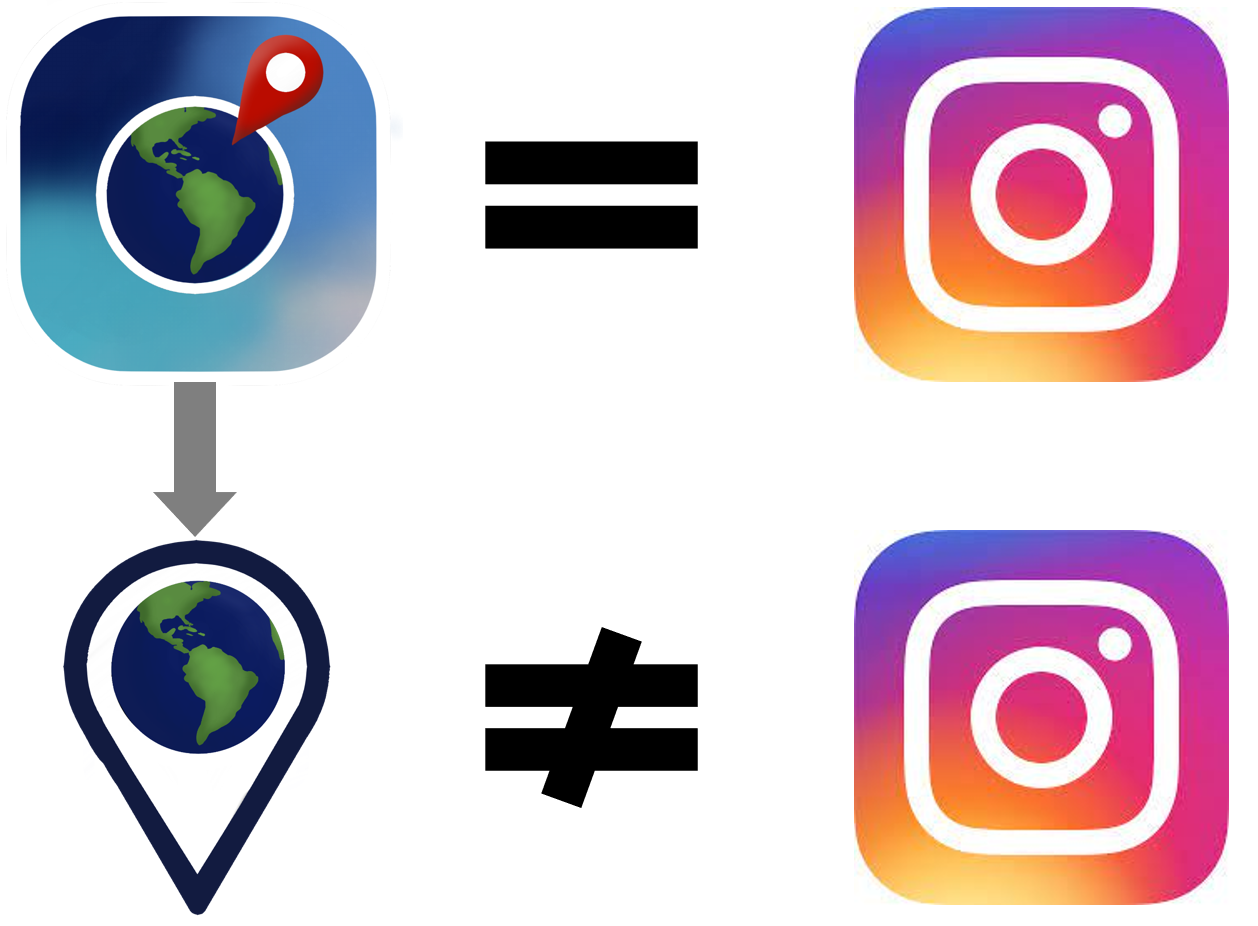
\includegraphics[width=0.8\linewidth]{images/logovsinsta.png}
    \caption{Übersicht der Logos}
    \label{fig:oldlogovsnewlogo}
\end{figure}

Neben dem Logo wurde zusätzlich noch der Name der App angepasst. Der bisherige Name \glqq Geogram\grqq{} wurde in den Namen \glqq GeoShare\grqq{} umgeändert. Grund ist die Ähnlichkeit der Namen \glqq Geogram\grqq{} und \glqq Instagram\grqq{}, bezüglich dem Teil \glqq \textbf{gram}\grqq{}.

Um die Veröffentlichung der App \glqq GeoShare\grqq{} im Google Play Store zu ermöglichen, waren noch zusätzliche Schritte notwendig. Wie in \autoref{fig:appinplaystore} zu erkennen, wurde die App mit dem Label \glqq \textbf{USK ab 18 Jahren}\grqq{} gekennzeichnet. Dies beruht auf der Tatsache, dass das Entwicklerteam keine Verantwortung über die hochgeladenen Inhalte übernimmt und potenzielle Benutzer auch kinderschädigende Bilder posten könnten.

Ebenso notwendig, war die Bereitstellung einer Datenschutzerklärung, welche vom Entwicklerteam zur Verfügung gestellt werden muss. Jene Datenschutzerklärung ist unter dem Link \glqq \url{https://datenschutz.dhbw-geogram.de/}\grqq{} zu finden.

\begin{figure}[H]
    \centering
    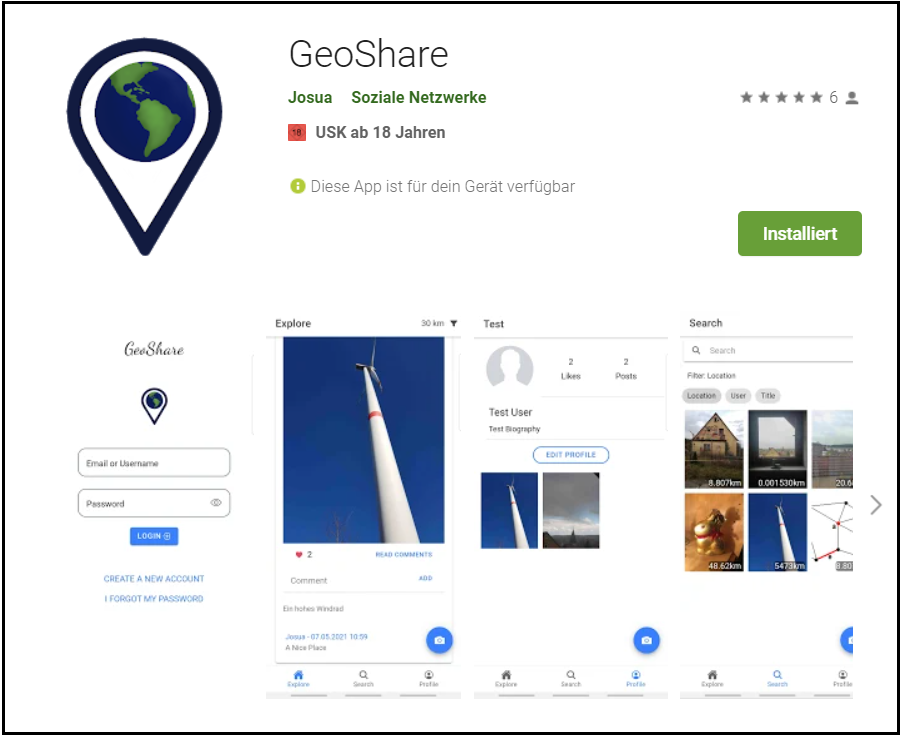
\includegraphics[width=0.9\linewidth]{images/playstore.png}
    \caption{Die App im Play Store}
    \label{fig:appinplaystore}
\end{figure}

Sollte das Entwicklerteam neue Features umsetzten, ist das Aktualisieren der App im Play Store mithilfe von Updates in wenigen Minuten möglich.